\documentclass[10pt]{jarticle}
\usepackage{ascmac}
\usepackage[dvipdfmx]{graphicx}
\usepackage{enumerate}
\usepackage{url}
\usepackage{listings}
\usepackage[hang,small,bf]{caption}
\usepackage[subrefformat=parens]{subcaption}
\renewcommand{\lstlistingname}{source}
\lstset{language=sh,%
        basicstyle=\footnotesize,%
	commentstyle=\textit,%
	classoffset=1,%
	keywordstyle=\bfseries,%
	frame=shadowbox,framesep=4pt,%
	showstringspaces=false%,
	numbers=left,stepnumber=1,numberstyle=\footnotesize,%
	numbersep=1zw,%
	lineskip=-0.5ex,%
	xleftmargin=2zw%
	}%

\newdimen\paperwidth \newdimen\paperheight
\def\A4size{\paperwidth=210mm \paperheight=297mm}
\def\centered{%
  \oddsidemargin=\paperwidth
  \advance\oddsidemargin-\textwidth
  \oddsidemargin=0.5\oddsidemargin
  \advance\oddsidemargin-1in
  \evensidemargin-\oddsidemargin}
%
\textwidth 160mm
\textheight 230mm
\topmargin 0mm
\headheight 0mm
\footskip 0mm
\A4size\centered

\title{\framebox{\hspace{4zw}データ科学 レポート1%
                 \hspace{4zw}}}
\author{神野 友哉 \\
        2022311042  \\
        愛知県立大学 情報科学部 情報科学科 \\}
\date{2023年12月4日}


\begin{document}
\maketitle

\section{課題 1}
\subsection{目的} \label{sec:hajime}
%
アムダール率\ r\ と、コア数\ N\ による理論上可能な速度向上度\ Sn\ の関係を可視化する
%

\subsection{方法} \label{sec:hoho}
%
以下のプログラム\ref{kadai1s}を実行する。
\begin{lstlisting} [caption=図\ref{fig:kadai1}のプログラム, label=kadai1s]
	clear;
	[r,n]=meshgrid(0:0.1:1,1:16);
	Sn=n./((n-1).*r+1)
	surf(r,n,Sn);colorbar;
	xlabel('r'),ylabel('n'),zlabel('Sn')
	print('wk1-1.pdf','-dpdf');
	hold off;
\end{lstlisting}
%

\subsection{実験結果} \label{sec:kekka}
%
結果、図\ref{fig:kadai1}となった。アムダール率\ r\ の値が十分小さい場合、理論上可能な速度向上度\ Sn\ は
コア数\ N\ と正の相関があるようにみえる。
%
\begin{figure}[htbp]
	\begin{center}
		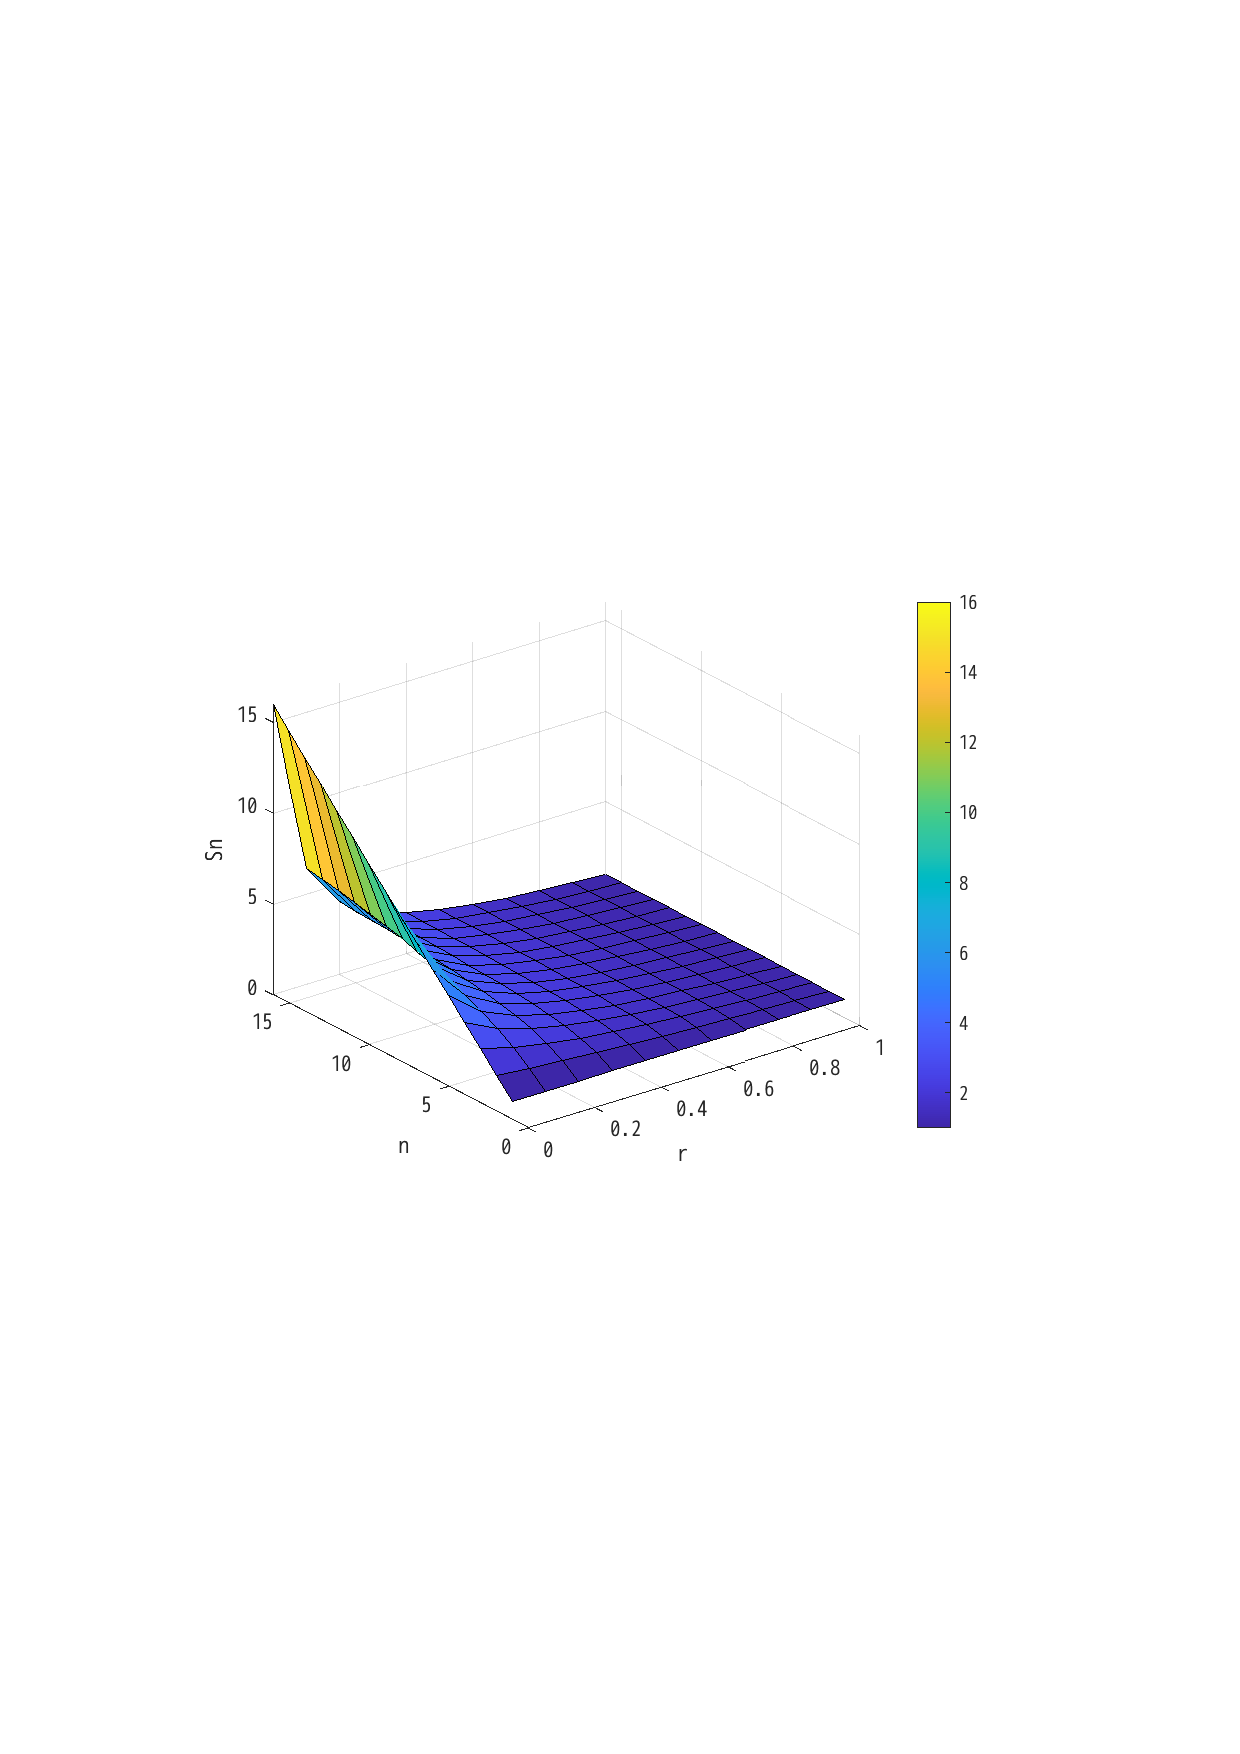
\includegraphics[width=70mm]{wk1-1.pdf}
	\end{center}
	\caption{Sn, r, Nの三次元描画}
	\label{fig:kadai1}
\end{figure}

\subsection{考察}
%
図\ref{fig:kadai1}から、プログラムの中でアムダール率\ r\ を低くする工夫を施さない限り、並列化\verb|(コア数 N)|による恩恵を得られづらいと考えられる。
それはアムダール率\ r\ の定義が、全体の実行時間の内、逐次処理できない部分の実行時間が占める割合\verb|(|$0\le r \le 1$\verb|)|であることからも解かる。
プログラムに施す具体的な工夫としては、\ parfor\ の外部で行う処理を減らす他に方法は無いと考えられる。
%

\subsection{感想}
%
図\ref{fig:kadai1}の\ 3Dplot\ の見た目が手前に寄っていたことが気になり、\ plot\ の向きを変更しようと試みたところ、今度は、軸の目盛りが見づらくなったため、
結局我慢した。
%

\section{課題 5}
\subsection{目的} \label{sec:5hajime}
%
並列化の影響を調査すること。
%

\newpage
\subsection{方法} \label{sec:5hoho}
%
\ N\ は並列化数\verb|(コア数)|である。\ matlab\ コマンドウィンドウから、\ parpool\verb|(N)|\ の\ N\ と
以下のプログラム\ref{kadai5s}の\ N\ の値を\ 1,\ 2,\ 4,\ 8,\ 16\ と各々変更→実行する。その後、コマンドウィンドウにて表示される
\ time,\ sn,\ Sn,\ en,\ En\ の値を記録する。そうして得られたデータに基づいて比較検証を行う。
\begin{lstlisting} [caption=モンテカルロ法にて円周率$\pi $を計算する際のプログラム, label=kadai5s]
	tic;
	nhist=1e7;
	count=0;
	time1=toc;
	tic;
	parfor i=1:nhist
		length=norm(rand(1,2));

		if (length<=1)
				count=count+1;
		end
	end

	time2=toc;
	tic;
	res=count/nhist*4
	res-pi
	time3=toc;

	N=4;
	amu=(time1 + time3) / (time1+time2+time3);
	amu
	Sn=1/(amu+(1-amu)/N);
	sn=5.7835/time2;
	En=sn/Sn;
	en=sn/N;
	time=time1+time2+time3;
	time
	sn
	Sn
	en
	En
\end{lstlisting}
%

\subsection{実験結果} \label{sec:5kekka}
%
結果は、表\ref{table:kadai5}のようになった。並列化数\verb|(コア数)|が増加するにつれて、並列化効率は減少している
ことが解かる。さらに、速度向上度\verb|(sn)|も、理論上の速度向上度\verb|(Sn)|に距離を大きく離されていくようだと解かる。
また、実行効率は並列化効率と近い値を取るようである。
%
\begin{table}[htbp]
	\centering
	\caption{モンテカルロ法にて円周率$\pi $を計算する際の処理並列化に伴う影響}
	\label{table:kadai5}
	\begin{tabular}{|c|c|c|c|c|c|}
		\hline
		並列化数\verb|(コア数)| & 実行時間\verb|(s)| & 速度向上度\verb|(sn)| & 理論上の速度向上度\verb|(Sn)| & 実行効率\verb|(en)| & 並列化効率\verb|(En)|\\
		\hline
		1  & 5.7835 & 1      & 1       & 1      & 1      \\
		2  & 3.1463 & 1.8382 & 1.9995  & 0.9191 & 0.9193 \\
		4  & 1.9369 & 2.9859 & 3.9952  & 0.7465 & 0.7474 \\
	  8  & 1.1574 & 4.9971 & 7.9581  & 0.6278 & 0.6279 \\
		16 & 0.8625 & 6.7059 & 15.7839 & 0.4191 & 0.4249 \\
		\hline
	\end{tabular}
\end{table}

\subsection{考察}
%
表\ref{table:kadai5}から、並列化数\verb|(コア数)|と並列化効率の関係を考察したい。
並列化数\verb|(コア数)|が\ 2\ の二乗で増加させているのにも関わらず、並列化効率は急激に減少する訳でもなく、緩やかに減少していると見える。
実際、それらの関係性を詳しく計算すると、以下の表\ref{table:kadai5n}であることが解かった。
特に、\ 並列化数\verb|(コア数)|\ 1\ に対する並列化効率\verb|(En)|の変位\ を見ると、コア数を増加させたとしても
、並列化効率はいづれ下げ止まると考えられる。要するに、コア数を無限に利用できる環境があったと仮定しても、並列化効率が
特定の値\ $\alpha$ \verb|(|$0\le \alpha \le 1 $\verb|)|\ に収束してしまい、無限の効率化を達成することはできないのではないか。
%
\begin{table}[htbp]
	\centering
	\caption{並列化数(コア数)の変位と並列化効率の変位の関係}
	\label{table:kadai5n}
	\begin{tabular}{|c|c|c|}
		\hline
		並列化数\verb|(コア数)|の変位 & 並列化効率\verb|(En)|の変位 & 並列化数\verb|(コア数)|\ 1\ に対する並列化効率\verb|(En)|の変位\\
		\hline
		1 - 2  & -0.0807 & -0.0807   \\
		2 - 4  & -0.1719 & -0.08595  \\
		4 - 8  & -0.1195 & -0.029875 \\
	  8 - 16 & -0.203  & -0.025375 \\
		\hline
	\end{tabular}
\end{table}

\subsection{感想}
%
電気の速度は光と同じか、もしくは若干劣る程度だと考えられている。しかし、電気の速度が光のそれを超えるような世界ならば、
更なる効率化を果たせたのではないかと、実験中のただ\ 5\ 分程度の休息時間に考えていた。
%

\end{document}
